\documentclass[a4paper,10pt]{article}
\usepackage[utf8]{inputenc}
\usepackage{amsmath}
\usepackage{amsfonts}
\usepackage{amssymb}
\usepackage{algorithm}
\usepackage[noend]{algpseudocode}
\usepackage{program}
\usepackage{amsmath}
\usepackage{graphicx}
\usepackage[T1]{fontenc}
\usepackage{eso-pic}
\usepackage{gensymb}
\usepackage{listings}
\usepackage{float}
\lstloadlanguages{R}

\newcommand{\BackgroundPic}{\put(-4,0){\parbox[b][\paperheight]{\paperwidth}{\centering
\includegraphics[width=\paperwidth,height=\paperheight]{nat-farve.pdf}}}}

\algnewcommand\True{\textbf{true}\space}
\algnewcommand\False{\textbf{false}\space}
\algdef{SE}[SUBALG]{Indent}{EndIndent}{}{\algorithmicend\ }%
\algtext*{Indent}
\algtext*{EndIndent}

\begin{document} 
	\AddToShipoutPicture*{\BackgroundPic}
	
	\begin{titlepage}
		\thispagestyle{empty}
		\vspace*{5cm}
		\begin{center}
			\Huge \textbf{Diskret Matematik og Algoritmer} \\
			\LARGE \textbf{Aflevering 8i} \\
		\end{center}
		\vspace*{3.5cm}
		\begin{flushleft}
			
		\begin{table}[h!]
			\begin{tabular}{lll}
				Adam Ingwersen,& \\ 
			\end{tabular}
		\end{table}
			
			
			\vspace{3mm}
			\vspace{3mm}
			Datalogisk  Institut\\
			Københavns Universitet\\
			\vspace{3mm}
			\today\\
			%\vspace*{0.5cm}
			
		\end{flushleft}
	\end{titlepage}

	\title{7g}
	\author{AAP}
	
	\newpage

\newpage

\section{}
\subsection{}
Denne delopgave følger kapitel 3 i KBR. 

For at danne en ordnet liste bestående af r elementer, der vælges fra en liste af 500 mulige elementer hvor gentagelser er tilladt er der følgende antal muligheder hvorpå dette kan gøres:
$$
500^{r}
$$

I det tilfælde, hvor gentagelser er tilladt, kan en ordnet liste bestående af \texttt{r} elementer med 500 mulige værdier, beskriver nedenstående formel antallet af muligheder:
$$
{}_{500}P_{r} = \frac{500!}{(500-r)!}
$$

\subsection{}
Det ønskes her at bestemme sandsynligheden for en kollision i tilfældet beskrevet i opgaveteksten. Det antages, at alle tilfælde er lige sandsynlige. Derfor kan sandsynlighedsfunktionen beskrives ved:
$$
p(n) = \frac{\frac{500!}{(500-n)!}}{500^n}
$$
Ved denne repræsentation, forventes det, at når \texttt{n} konvergerer mod 500, vil $p(n)$ ligeledes konvergere mod $1$ - altså bliver kollisioner gradvist mere sandsynlige - og ved 500, uundgåelige. Dette jf. skuffeprincippet. Omvendt, vil et lille \texttt{n} betyde en lav sandsynlighed for kollisioner. 
Grænseværdierne for \texttt{n} betragtes:
$$
p(500) = \frac{\frac{500!}{(500-500)!}}{500^{500}} = 0
$$
$$
p(0) = \frac{\frac{500!}{(500-0)!}}{500^0} = 1
$$
Her er sandsynlighedsfunktionen $p(n)$ monotont aftagende.

\newpage

\subsection{}
Givet at fakultets-funktionen, under normale omstændigheder, er en integer-funktion - vil det her ikke forsøges at identificere decimal-værdien, hvor $y = 0.5$, men her angives et heltal i stedet. Den første værdi for \texttt{n}, hvortil sandsynligheden for ingen kollision er under \texttt{0.5} er \texttt{27}.

Sandsynlighedsfunktionen samt en effektivisering af permutations-funktionen er angivet i R-kode i bilag sammen med kode, der genererer et plot. 

\begin{figure}[H]
\centering
\caption{Sandsynlighedsfunktionen fra \texttt{n = 1..100}}
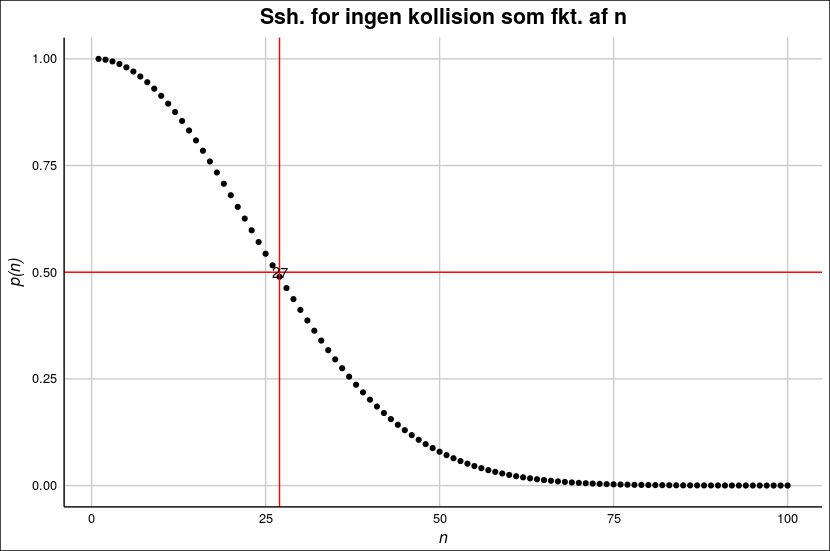
\includegraphics[scale = 0.45]{plot.png}
\end{figure}

\section{}
\subsection{}
\subsubsection*{Refleksivitet}
R er refleksiv, da:
$$
xRx \forall x \in \mathbb{R}
$$

\subsubsection*{Symmetri}
R er symmetrisk, da hvis det gælder, at $x-y \in \mathbb{Z}$, vil det ligeldes gøre sig gældende, at $y-x \in \mathbb{Z}$
\subsubsection*{Transitivitet}
Antag, at $xRy \in \mathbb{Z}$ og $yRz \in \mathbb{Z}$, da lades:
$$
x - y = k_{1} \in \mathbb{Z}
$$
$$
y - z = k_{2} \in \mathbb{Z}
$$
Da må:
$$
k_{1} + k_{2} = x - y + y - z = x - z \in \mathbb{Z}
$$
Altså, er R en Transitiv relation.

\subsection{}
\subsubsection*{Refleksivitet}
S er ikke refleksiv i de tilfælde, hvor $x = 0$ altså:
$$
xRx \ngtr 0 \forall x = 0
$$

\subsubsection*{Symmetri}
S er symmetrisk, da multiplikationsrelationen i sig selv er symmetrisk - enhver relation, S, hvor $x\cdot y > 0$, vil det ligeledes gælde, at $y\cdot x > 0$.
\subsubsection*{Transitivitet}
S er transitiv, da der ved multiplikation aldrig vil opstå en situation, hvor relationen ikke er opfyldt i $x\cdot z$, hvis og kun hvis relationen er overholdt for $x\cdot y$ samt $y\cdot z$. For at $x\cdot y > 0$, da må $x$ og $y$ have samme fortegn. Det samme gælder for $y \cdot z$, hvorved det må gælde, at $x$ og $z$ begge har samme fortegn. Så må $xRz > 0$, hvis $xRy \wedge yRz > 0$. 

\newpage

\section*{Bilag}
\subsection*{R Kode}
\lstinputlisting[language=R]{perm.R}

\end{document}
